\newpage
\subsection{Turn-Minimizing Reach Set Approximation}\label{s:harmonicReachSet}

\paragraph{Summary:} This procedure will produce trajectories minimizing aggressive maneuvering, ideal for navigation tasks.

\paragraph{Motivation:} Imagine having an \emph{Avoidance Grid} like (fig. \ref{fig:LidarSpaceSegmentation}). There is a need of \emph{Reach Set Approximation} which will have \emph{Smooth Trajectories} (def. \ref{def:SmoothnessRatingForTrajectory}) going nearby $cell$ centers.

\paragraph{Background:} The \emph{Smoothness Rating for Trajectory} (def. \ref{def:SmoothnessRatingForTrajectory}) uses two distinct sets \emph{Smooth Movements} and \emph{Chaotic Movements} (eq. \ref{eq:ChaoticSmoothMovementSetDefinition}) which are defined for our \emph{Movement Automaton}  (sec. \ref{s:modelMAImplementation}) like the following:

\begin{equation}
    \begin{aligned}
    Smooth Movements &= \{Straight\} \\
    Chaotic Movements &= Movements - Smooth Movements\\
    \end{aligned}
\end{equation}

\emph{Smooth Movements} contains only \emph{Straight} movement because others are considered as extreme turning movements. \emph{Smooth Movements} should contain only direct flight movements or slight heading correction. \emph{Chaotic Movements} set is a  supplement of \emph{Movement Automaton`s Movement Set}. 

The \emph{Avoidance Grid} (fig. \ref{fig:LidarSpaceSegmentation}) cell centers for fixed indexes $j_{fix}$, $k_{fix}$ are linearly aligned with the \emph{initial state}. That means that  cell centers of cells $cell_{1,j_{fix},k_{fix}},\dots, cell_{i,j_{fix},k_{fix}}$, where $i$ is a count of \emph{layers} lie on one line.  If the trajectory can achieve \emph{cell center} on some \emph{layer}, only minor trajectory corrections are required to stay on the given line. This type of trajectory gives us the  following advantages:
\begin{enumerate}
    \item\emph{Minimal steering at the beginning} - the minimal steering is advantageous in \emph{Controlled Airspace} because is diminishing the amount of communication to \emph{UTM Service}.
    
    \item\emph{Additional safe space in the linear segment} - once the \emph{center of the cell} is reached, \emph{Trajectory} sticks to the line between cell centers. Each point on this line has the \emph{maximal distance} to outer walls of the cell. This gives us extra space given as minimum of distance between \emph{UAS position} and \emph{Outer cell walls}.
\end{enumerate}

\paragraph{Expansion Constraint Function Implementation} (alg. \ref{alg:ExpansionConstraintFunctionForHarmonicReachSet}) is based on the simple principle: \emph{Select candidate Nodes  which are closest to Cell center, with a unique footprint}.

\begin{note}
    \emph{Cell center} can be closely reached by \emph{smooth movement} from a previous cell or \emph{chaotic movement} from a neighboring cell from the current or previous layer. These trajectories are usually equivalent in \emph{Smoothness}.
\end{note}

\begin{algorithm}[H]
\SetKwInOut{Input}{Input}\SetKwInOut{Output}{Output}\SetKwInOut{TuningParameters}{Tuning Parameters}
    \Input{Node[] stack, Cell cell$_{i,j,k}$}
    \TuningParameters{int$^+$ spreadLimit}
    \Output{Node[] candidates, Node[] leftovers}
    
    \BlankLine
    \# Initialize structures\;
    Node[] candidates = [], Node[] leftovers=[]\;
    Node[] passing = cell$_{i,j,k}$.getFinishingTrajectories(stack)\;
    
    \BlankLine
    \# Select unique smoothest trajectories\;
    Map$<$Buffer,Node$>$  bestPerformanceMap\;
    \For{Node test $\in$ passing}{
        centerDistance= test.getPerformance(cell$_{i,j,k}$)]\;
        footPrint = test.getFootprint()\;
        \eIf{bestPerformanceMap.contains(footPrint)}{
            old = bestPerformanceMap.getByKey(footprint)\;
            oldPerformance= old.getPerformance(cell$_{i,j,k}$)\;
            \If{oldPerformance $>$ centerDistance}{
                bestPerformanceMap.setByKey(footprint,test)\;         
            }
        }{
            bestPerformanceMap.setByKey(footprint,test)\;
        }
    }
    
    \BlankLine
    \# Select best performing nodes up to \emph{spreadLimit} count\;
    candidates = bestPerformanceMap.select(count = spreadLimit).orderBy('cellCenterDistance','Ascending')\;
    leftovers = passing - candidates\;
    \Return{[candidates,leftovers]}
    
    
    \caption{Expansion Constraint function for \emph{Turn-Minimizing Reach Set Approximation}}
    \label{alg:ExpansionConstraintFunctionForHarmonicReachSet}    
\end{algorithm}


\paragraph{Tuning Parameter:} \emph{Proximity to Cell Center} gives a good chance to keep trajectory smooth or \emph{smooth after one correction maneuver}. It has been mentioned that \emph{Cell Center} can be reached by various trajectories. In this method full footprint length is always considered; therefore only one tuning parameter can be offered:
\begin{enumerate}
    \item \emph{Spread Limit} - the upper limit of candidates which are going to be selected for further expansion, minimal value 1, default value \emph{Count of unique Moves in Movement set}, the maximal value $\infty$. If maximal value $\infty$ is selected, the algorithm will generate the skeleton of \emph{Reach Set} with full Coverage and with the smoothest \emph{Trajectories}.
\end{enumerate}

\paragraph{Step: Initialization} sets candidate \emph{Nodes} as empty set, leftover \emph{Nodes} as empty set. and selects all \emph{Nodes} from \emph{Stack} which represents  \emph{Finishing Trajectories} in working cell $cell_{i,j,k}$.

\paragraph{Step: Evaluate smoothest trajectories with unique Footprints} is implemented as \emph{multi-criteria filtration}. 

The \emph{first criterion} is the \emph{distance to Cell Center} which is penalized by trajectory \emph{smoothness rate} implemented in method \emph{Node.getPerformance(Cell $cell_{i,j,k}$)} defined as follow.

\begin{equation}
    getPerformance(Node,Cell) = \frac{distance(Node.Trajectory,Cell.Center)}{SmoothnessRate(Node.Trajectory)}
\end{equation}

\noindent Distance of \emph{Trajectory} is \emph{enumerator} because its considered as the \emph{base value} and is defined in the interval $[0,maximalWallDistance]$. The \emph{Smoothness Rate} is the denominator, because it is a penalization coefficient defined in the interval $[0,1]$. 

The \emph{second criterion} is \emph{trajectory uniqueness}. This is provided by \emph{Best Performance Map}, where best performing \emph{Node} belongs to one unique \emph{trajectory footprint}. The implementation is identical to \emph{coverage-maximizing set expansion} (alg. \ref{alg:ExpansionConstraintFunctionForChaoticReachSet}).

\paragraph{Step: Select candidates} is executed  on \emph{Best Performance Map} records using \emph{Penalized Cell Center Distance} as pivot parameter, ordered in ascending order and limited by \emph{Spread Limit} tuning parameter. The \emph{Leftovers} are difference set between \emph{Passing Nodes} and \emph{Candidate Nodes}.




\paragraph{Example:} for \emph{Avoidance Grid} with \emph{Distance 10 m}, \emph{Layer count 10}, \emph{Horizontal range $[-45^\circ,+45^\circ]$}, \emph{Horizontal Cell Count 7}, \emph{Vertical range $[-30^\circ,+30^\circ]$}, and \emph{Vertical Cell Count 5}. Is given in (fig. \ref{fig:harmonicReachSetApproximation}). The UAS is at \emph{Back-side} of \emph{Figure} (the initial state is at all \emph{Trajectory Origins}). The \emph{black dashed line} marks \emph{Avoidance Grid} space boundary. Each trajectory has its color and ends at \emph{Front-side} of \emph{Avoidance Grid Boundary}. The \emph{Spread Limit}, in this case, was set to $9$ which is \emph{Size of the Movement Set}.

\begin{note}
    Please note \emph{Trajectories} are organized in bundles going around \emph{Cell Centers smoothly}. Most of the steering maneuvers are executed at the \emph{beginning} of the \emph{Avoidance Grid}.
\end{note}

\begin{figure}[H]
    \centering
    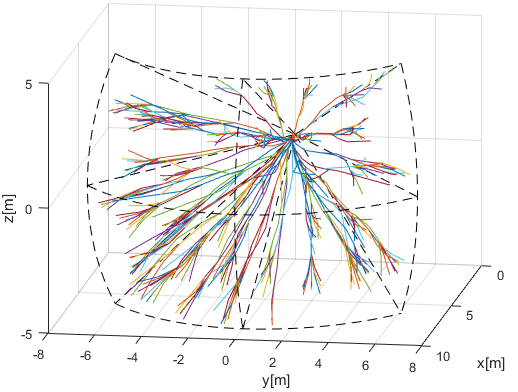
\includegraphics[width=0.7\linewidth]{\FIGDIR/RS003HarmonicReachSetEstimationMethod} 
    \caption{\emph{Turn-minimizing \emph{reach set} approximation}.}
    \label{fig:harmonicReachSetApproximation}
\end{figure}

\paragraph{Pros and Cons:} It can be seen from example (fig. \ref{fig:harmonicReachSetApproximation}) that \emph{Turn-Minimizing Reach Set Approximation Method} (alg. \ref{alg:ExpansionConstraintFunctionForHarmonicReachSet}) generates \emph{smooth evenly spread trajectories}.
    
High smoothness ratio ($\ge 0.9$) is provided while keeping low node count for UAS systems. The calculation complexity scales linearly with grid size. The upper limit of trajectories is given as follow:

\begin{equation}
    countTrajectories(ReachSet) \le layerCellCount \times spreadLimit \times size(Movements)
\end{equation}

\noindent The \emph{upper limit of nodes} is given as follow:

\begin{equation}
    countNodes(ReachSet) \le layerCount \times layerCellCount \times spreadLimit
\end{equation}

\noindent The absence of \emph{High Coverage Ratio} disqualifies \emph{Turn-Minimizing Reach Set Approximation} to be used for \emph{Emergency Avoidance}. This type of \emph{Reach Set} is feasible for \emph{Open Space Navigation} or \emph{Controlled Airspace Navigation}. Its low turning rate in contained \emph{Trajectories} are desired for such tasks. 



